\documentclass[a4paper, twocolumn]{article}
\newcommand{\spc}{\vspace{5mm}}

\usepackage[utf8]{inputenc}
\usepackage[T1]{fontenc}
\usepackage[spanish]{babel}

\usepackage{amsmath}
\usepackage{graphicx}
\usepackage{hyperref}
\usepackage{amssymb}
\usepackage{color}
\usepackage{listings}
\usepackage{times}

\graphicspath{ {images/} }


\begin{document}

\title{Formulario Finanzas}
\author{Sebastián Lévano}
\date{\today}
\maketitle

% \section{Tiempo}

% \begin{figure}
%     \centering
%     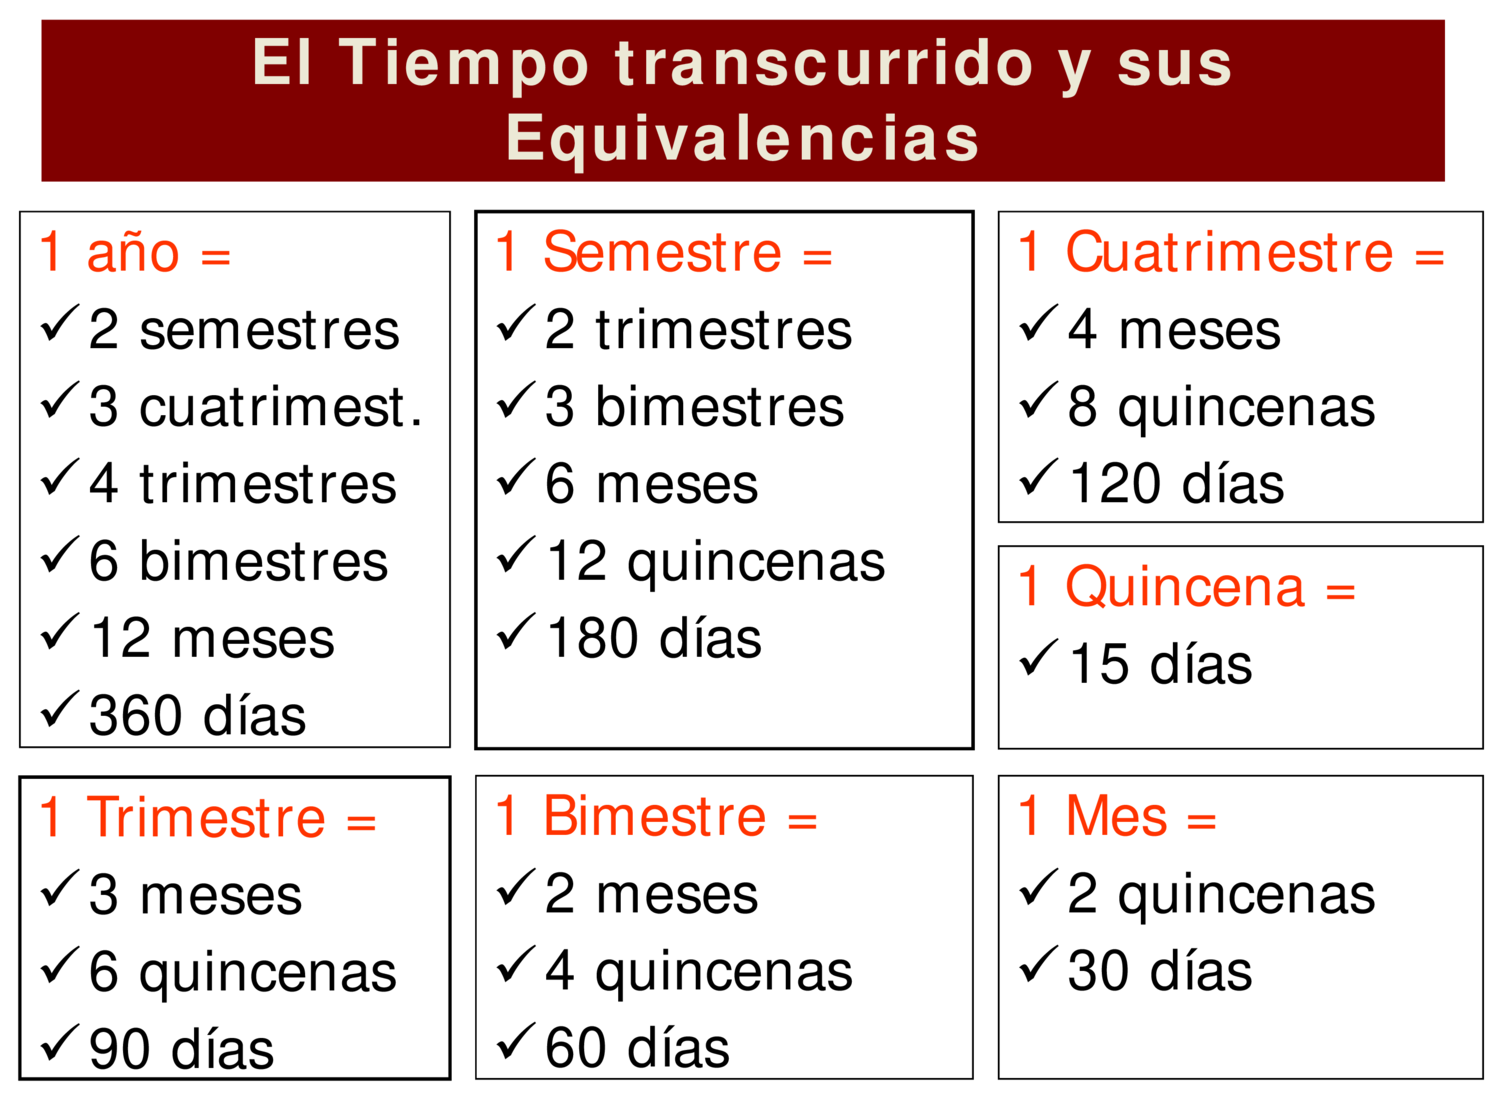
\includegraphics[scale=0.33]{Tiempo_Equivalencias}
% \end{figure}

% \begin{figure}
%     \centering
%     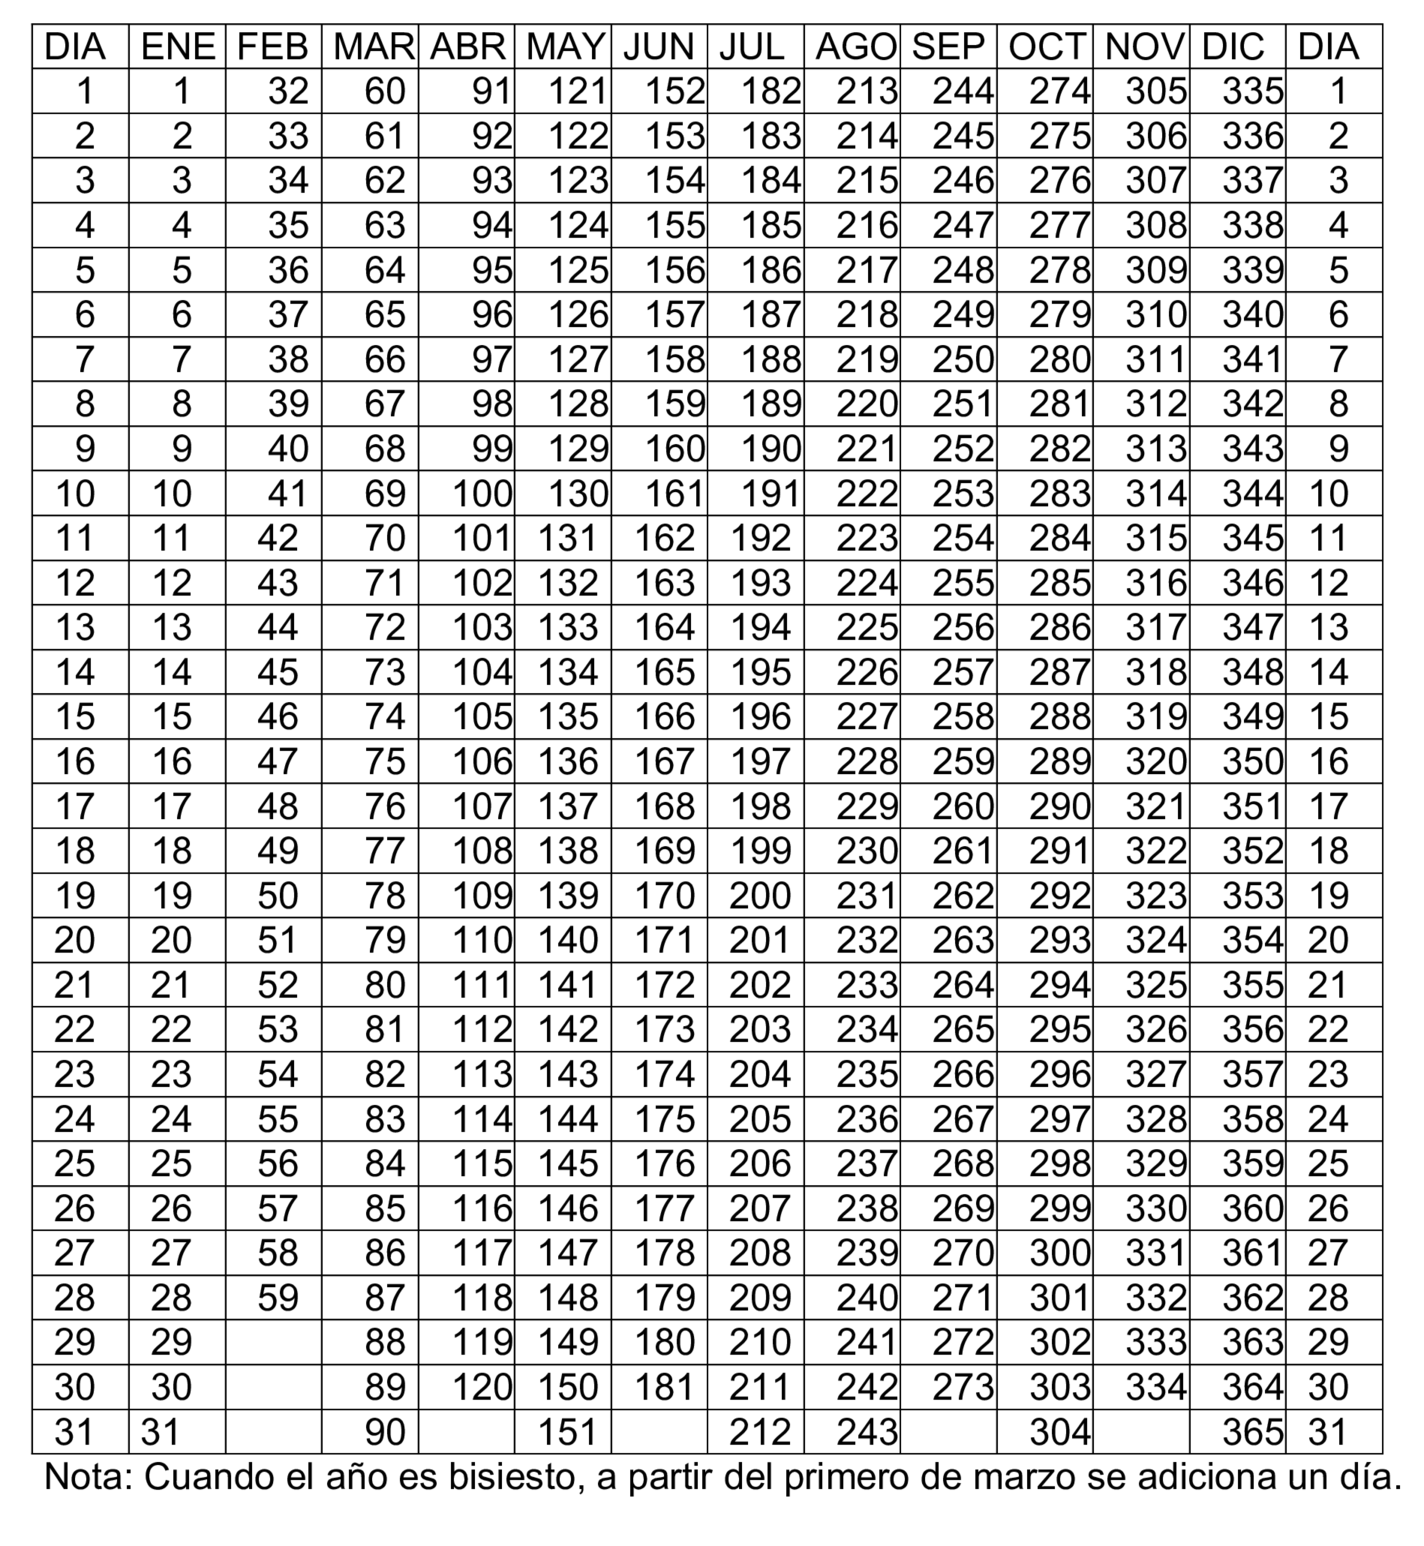
\includegraphics[scale=0.35]{Tabla_Dias}
% \end{figure}

\section{Interés Simple}

\begin{gather*}
    I = S - C \\
    I = C \cdot i \cdot t \\
    S = C \cdot (1 + i \cdot t) \\
    C = \frac{S}{(1 + i \cdot t)} \\
    C = S \cdot (1 + i \cdot t)^{-1} \\
    D = d \% C \\
    i = \frac{(\frac{S}{C} - 1)}{t} \cdot 100 \% \\
    Saldo = C - D \\
    P_l = P_c + recargo \% \cdot P_c \\
    C = P_c - C_i \\
    S = P_l - C_i
\end{gather*}

Donde:

\begin{align*}
    I = \text{Interés}                                \\
    S = \text{Stock - Monto - Valor Futuro}           \\
    C = \text{Capital - Valor Presente}               \\
    i = \text{Tasa de interés}                        \\
    t = \text{Tiempo}                                 \\
    (1 + i \cdot t) = \text{Factor de acumulación}    \\
    \text{a tasa de interés simple}                   \\
    (1 + i \cdot t)^{-1} = \text{Factor de descuento} \\
    \text{a tasa de interés simple}                   \\
    P_l = \text{Precio de lista}                      \\
    P_c = \text{Precio de venta - Precio al contado}  \\
\end{align*}


\section{Interés Nominal}


\begin{gather*}
    i' = \frac{TN}{m} \\
    TEP = (\frac{S}{C} - 1) \cdot 100 \% \\
    S = C \cdot (1 + i')^n \\
    S = C \cdot (1 + \frac{TN}{m})^n \\
    C = \frac{S}{(1 + \frac{TN}{m})^n} \\
    C = S \cdot {(1 + \frac{TN}{m})^{-n}} \\
    n = \frac{\ln{\frac{S}{C}}}{\ln{(1 + \frac{TN}{m})}} \\
    TN = m \cdot (\sqrt[n]{\frac{S}{C}} - 1) \cdot 100 \% \\
\end{gather*}

Donde:

\begin{align*}
    I = \text{Interés}                                \\
    S = \text{Stock - Monto - Valor Futuro}           \\
    C = \text{Capital inicial - Valor Presente}       \\
    i' = \text{Tasa de interés}                       \\
    \text{en el periodo de capitalización}            \\
    TN = \text{Tasa nominal}                          \\
    TEP = \text{Tasa efectiva anual}                  \\
    t = \text{Tiempo}                                 \\
    n = \text{Número de periodos}                     \\
    m = \text{Número de veces}                        \\
    \text{que se repite el periodo de capitalización} \\
\end{align*}

\subsection{Recordatorios}

\begin{itemize}
    \item Todos los tiempos se rigen por la capitalización.
    \item La $TEP$ se haya en abse al tiempo.
          Ejemplo: $t = 6$ meses, entonces se haya una $TES$
\end{itemize}

\section{Interés Efectivo}

\begin{gather*}
    TEP = (\frac{S}{C} - 1) \cdot 100 \% \\
    TEP = ((1 + \frac{TN}{m})^n - 1) \cdot 100 \% \\
    TN = m \cdot (\sqrt[n]{1 + TEP} - 1) \cdot 100 \% \\
    TEP_2 = (1 + TEP_1)^{\frac{n_2}{n_1}} - 1) \cdot 100 \% \\
    S = C \cdot (1 + TEP)^n \\
    S = C \cdot (1 + TEP)^{\frac{\text{Nro días trasladar}}{\text{Nro días TEP}}} \\
    C = \frac{S}{(1 + TEP)^{\frac{\text{Nro días trasladar}}{\text{Nro días TEP}}}} \\
    n = \frac{ln{\frac{S}{C}}}{ln{1 + TEP}} \cdot {\text{Nro días TEP}} \\
    TEP = (\frac{S}{C})^{\frac{\text{Nro días TEP}}{\text{Nro días trasladar}}} - 1 \\
\end{gather*}

Donde:

\begin{gather*}
    m = \text{Número de capitalizaciones de la Tasa Nominal} \\
    \text{en el tiempo que quedo expresada} \\
    n = \text{Número de capitalizaciones realizadas} \\
    \text{en el tiempo de la inversión} \\
\end{gather*}

\section{Tasa Descontada}

\begin{gather*}
    \text{Descuento} = \text{Valor Nominal} \cdot d\% \\
    \text{Valor Neto} = \text{Valor Nominal} - \text{Descuento} \\
    \text{Valor Neto} = \text{Valor Nominal} \cdot (1 - d\%) \\
    d\% = \frac{i'}{1 + i'} \\
    i' = \frac{d\%}{1 - d\%} \\
    \text{Valor Neto} = \text{Valor Nominal} \cdot (1 + TE)^{\frac{nd}{n}} \\
    TEtd = (1 + \frac{TN}{m})^n - 1 \\
    TEtd = (1 + TEP)^\frac{td}{n} - 1 \\
    dt = \frac{TEtd}{1 + TEtd} \\
    d\% = dt \\
    \text{Valor recibido} = \text{Valor Neto} - \text{Suma de los costes} \\
    \text{iniciales} - \text{Retención} \\
    \text{Valor entregar / cancelar} = \text{Valor Nominal} + \text{Suma de} \\
    \text{los costes finales} - \text{Retención} \\
    TCEA = \frac{\text{Valor Entregado}}{\text{Valor Recibido}}^\frac{360}{td} - 1 \\
\end{gather*}

Donde:

\begin{gather*}
    i' = \text{Tasa Efectiva en el Período de descuento (TEP)} \\
    d\% = \text{Tasa de Descuento equivalente} \\
    nd = \text{Número de días de descuento} \\
    n = \text{Número de días del período de descuento} \\
    td = \text{Tiempo transcurrido desde la fecha del descuento} \\
    TEtd = \text{Tasa Efectiva en el período de tiempo} \\
    \text{transcurrido} \\
    TCEA = \text{Tasa de Coste Efectivo Anual} \\
\end{gather*}

\end{document}
